\newcommand{\code}{\texttt}

\chapter{Úvod}
Moderné procesory od výrobcu \emph{Intel} majú na svojich čipoch integrované obvody a čítače pre počítanie a ukladanie odhadu spotreby niektorých častí procesora.
Prístup k týmto čítačom bol pôvodne neprivilegovaný, čo otváralo možnosti potenciálnych postranných útokov, na základe čoho bola rodina útokov
Platypus vyvinutá. Jedná sa o plne softvérové útoky, ktorými je možné extrahovať rôzne citlivé informácie z napadnutého systému. Medzi samotné útoky
patrí rozlišovanie vykonávaných inštrukcií a veľkostí ich operandov, získanie RSA kľúča zo \emph{square-and-always-multiply} algoritmu a mnoho ďalších.

\chapter{Platypus}
%\section{Intel RAPL} \label{sec:rapl}
Moderné \emph{Intel} procesory poskytujú \emph{RAPL} (Running Average Power Limit) rozhrania pre monitorovanie odhadovanej akumulovanej spotreby procesora
od jeho resetu. Táto spotreba je ukladaná v modelu špecifických registroch (MSR) a je ju možné čítať priamo (rozhrania \code{/dev/msr}, \code{/dev/safe-msr}
alebo \code{/dev/cpu/*/msr}),
prípadne za pomoci rámca \code{powercap}. Týmto spôsobom meraná spotreba je často využívaná pre rôzne účely ako sú modulácia výkonu procesora,
sledovanie spotreby, prípadne profilovanie softvéru.
RAPL poskytuje údaje pre rôzne domény procesora:
\begin{itemize}
    \item \emph{core} pre konkrétne jadro procesora,
    \item \emph{uncore} pre integrované grafické čipy apod.,
    \item \emph{package} zahŕňajúci core a uncore domény,
    \item \emph{DRAM} pre systémovú pamäť pre daný soket.
\end{itemize}
Toto rozdelenie platí pre väčšinu procesorov, avšak niektoré nové procesory obsahujú viac, než jednu package doménu na jednom čipe, prípadne sa dopĺňa
nová doména \emph{psys}\footnote{\href{https://github.com/powercap/powercap/issues/3}{https://github.com/powercap/powercap/issues/3}}.
Rámec \code{powercap} umožňuje jednoduchý prístup k týmto doménam.
RAPL registre sa podľa zistení \cite{Platypus} aktualizujú raz za $1000 \mu s$ pre domény package a DRAM a raz za $50 \mu s$ pre doménu core.
Časy pre domény core a package boli zmerané aj mojou implementáciou a žiadny zásadný rozdiel v rýchlosti aktualizácie hodnôt
nebol na testovanom systéme zaznamenaný - obe domény sa aktualizovali raz za približne $1000 \mu s$, rovnako ako je uvedené v Intel referenčnom
manuáli \cite{intel_manual}.

\section{Analýza výkonu}
V niektorých prípadoch je na hardvéri možné vykonávať postrannú analýzu systému fyzicky. Takéto prístupy vyžadujú špeciálne pomôcky,
ktoré majú vysokú vzorkovaciu frekvenciu, vďaka čomu je často možné získať dostatočné množstvo dát o systéme v rámci jednej alebo
iba niekoľkých \emph{stôp}\footnote{Stopa (angl. trace) je množina hodnôt získaných počas analýzy.}.
Takáto analýza sa nazýva \emph{SPA} (angl. Simple Power Analysis) a pre účely tejto práce nie je vhodná.

Typ analýzy \emph{DPA} (angl. Differential Power Analysis) využíva veľké množstvo získaných stôp, na ktorých je vykonaná štatistická analýza.
Výhodou tejto metódy je schopnosť spriemerovať šum, vďaka čomu sa môžu detegovať aj veľmi malé výchylky v spotrebe \cite{Platypus}. V niektrých prípadoch sú tieto
výchylky spôsobované napríklad operandami inštrukcií, ktoré nie sú pomocou SPA ľahko (alebo vôbec) detegovateľné. Prístup DPA je vhodný aj pre
prípady, keď je vzorkovacia frekvencia výrazne obmedzená.

\section{Experimenty}
Táto práca sa pokúsila reprodukovať niektoré časti publikácie \cite{Platypus}.
Procesor, na ktorom boli vykonávané experimenty je \emph{Intel Core i5-4200U CPU @ 1.60GHz} (architektúra \emph{Haswell}). Bola využitá knižnica
powercap\footnote{Knižnica powercap \href{https://github.com/powercap/powercap}{https://github.com/powercap/powercap}.} pre čítanie RAPL registrov
a implementácia rozhrania pre čítanie TSC (Time Stamp Counter) registra\footnote{Rozhranie pre čítanie TSC registra\\\href{https://github.com/LITMUS-RT/liblitmus/blob/master/arch/x86/include/asm/cycles.h}{https://github.com/LITMUS-RT/liblitmus/blob/master/arch/x86/include/asm/cycles.h}.}.
Obrázky a tabuľky sú zostavované podobne ako v \cite{Platypus} pre referenciu a porovnanie získaných výsledkov.

\subsection{Analýza spotreby energie pre jednotlivé inštrukcie}
Spotreba energie inštrukcií bola meraná pomocou RAPL rozhrania, čo znamená, že vzorkovacia frekvencia je prinízka pre meranie spotreby jedného spustenia inštrukcie.
Ako kompenzácia pre túto skutočnosť sa každá inštrukcia spúšťala $50000$-krát po sebe a bola zmeraná celková spotreba od začiatku behu po koniec. Tieto spustenia
boli zabalené do cyklu, čím sa ale pridala nežiadaná réžia do merania. Vplyv na spotrebu energie tejto réžie bol odstránený odpočítaním zmeranej spotreby
prázdneho cyklu od získaných meraní pre inštrukciu. Spotreba bola takto pre každú inštrukciu meraná toľkokrát, kým sa nezískalo $10000$ nenulových stôp.
Ošetrenie pre prijatie iba nenulovej stopy je z dôvodu, že pri mnohých inštrukciách, ktorých rýchlosť vykonania je privysoká, sa RAPL čítače nestihnú aktualizovať.

\begin{figure}\label{img:instruction_comparison}
  \centering
  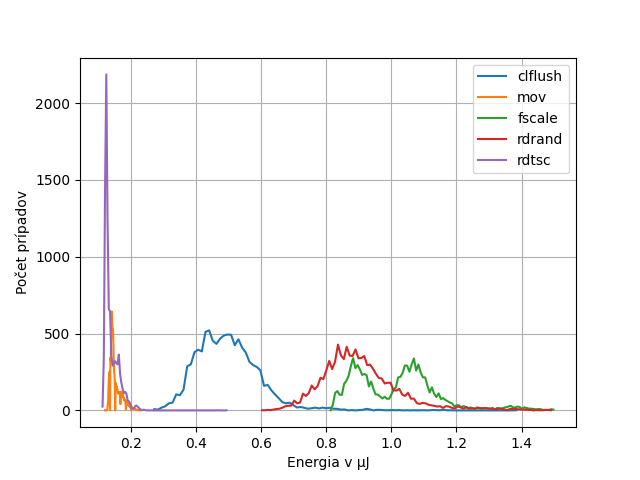
\includegraphics[scale=0.7]{./obrazky-figures/instr_comparison.png}
  \caption{Porovnanie spotreby vybraných inštrukcií.}
\end{figure}

Na obrázku \ref{img:instruction_comparison} je zobrazená energetická spotreba vybraných inštrukcií. V porovnaní s \cite{Platypus} je možné vidieť nielen odlišné
zoradenie inštrukcií podľa spotreby, ale aj rôzne prekrytie spotrieb. Inštrukcia \code{clflush} je najjednoduchšie rozlíšiteľná od ostatných, pričom \code{rdtsc} sa
od \code{mov} líši minimálne. Tabuľka \ref{tab:avg_energy_per_instruction} zobrazuje priemernú zmeranú spotrebu pre deväť rôznych inštrukcií.

\begin{table}\label{tab:avg_energy_per_instruction}
  \centering
  \caption{Priemerná zmeraná spotreba jednotlivých inštrukcií.}
  \begin{tabular}{ | l  r | }
    \hline
    Inštrukcia & Priemerná spotreba \\
    \hline
    \code{nop} & $0.08901 \mu J$ \\
    \code{inc} & $0.09315 \mu J$ \\
    \code{xor} & $0.09298 \mu J$ \\
    \code{mov} & $0.18403 \mu J$ \\
    \code{imul} & $0.17493 \mu J$ \\
    \code{fscale} & $1.10859 \mu J$ \\
    \code{rdrand} & $1.03944 \mu J$ \\
    \code{rdtsc} & $0.16500 \mu J$ \\
    \code{clflush} & $0.46188 \mu J$ \\
    \hline
  \end{tabular}
\end{table}

\subsection{Analýza spotreby energie pre rôzne operandy}
Podobne ako pri meraní spotreby inštrukcií, aj tu sa inštrukcie spúšťali $50000$-krát, avšak samotných stôp sa získavalo až $70000$.
Merala sa inštrukcia \code{imul}, pre ktorú sa podobne ako v \cite{Platypus} nastavil jeden operand na konštantu $8$, pričom druhý
sa nastavil na tri rôzne Hammingove váhy, konkrétne na $0$, $32$ a $64$. Bity operandov boli nastavené zoskupene, a teda jeden sled núl nasledovaný jedným sledom
jednotiek. Na obrázku \ref{img:imul_operands} je vidieť, že veľkosť operandov nemá žiaden výrazný dopad na rozloženie spotreby energie čítanej pomocou RAPL.

\begin{figure}\label{img:imul_operands}
  \centering
  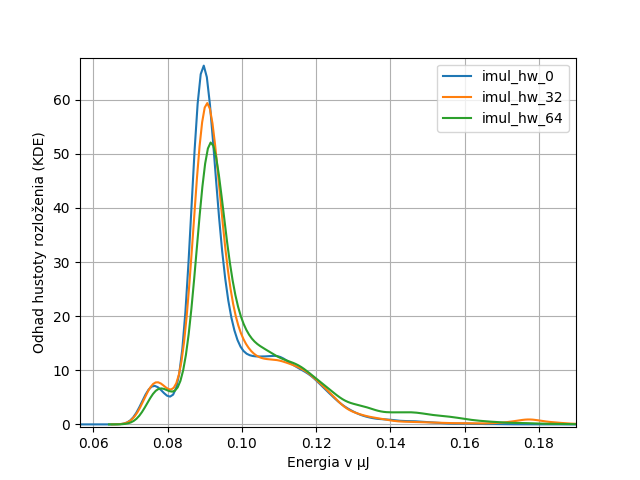
\includegraphics[scale=0.7]{./obrazky-figures/imul_operand_consumption.png}
  \caption{Porovnanie spotreby inštrukcie \code{imul} s operandami rôznej Hammingovej váhy.}
\end{figure}

\subsection{Skrytý kanál}
Jednou z vecí, ktoré monitorovanie spotreby procesora umožňuje, je vytvorenie skrytých kanálov za pomoci manipulácie spotreby. Na obrázku \ref{img:covert_channel}
je možné vidieť vizualizáciu správy zaslanej cez skrytý kanál medzi dvoma procesorovými vláknami. Zasielaná správa bol sled bitov \code{101001100}.
Vlákna neboli žiadnym spôsobom explicitne synchronizované, kvôli čomu je možné vidieť kľudový stav spotreby pred prvým preneseným bitom, ked prijímač iba naslúchal.

Počas implementácie skrytého kanálu sa prejavilo možné obmedzenie knižnice powercap, a to také, že nie je schopné získať informácie o spotrebe energie v prípade,
že je volaná v rámci dynamicky vytvoreného vlákna. Kvôli tomuto obmedzeniu sa pre účely merania spotrebovanej energie pristupovalo priamo k MSR cez
rozhranie \code{/dev/cpu/*/msr}.

\begin{figure}\label{img:covert_channel}
  \centering
  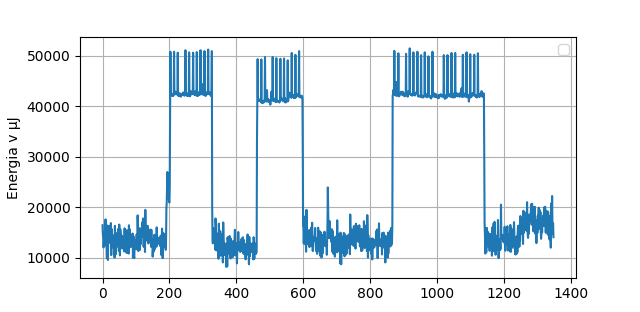
\includegraphics[scale=0.7]{./obrazky-figures/covert_channel.png}
  \caption{Vykreslenie sledu bitov \code{101001100} poslaných cez skrytý kanál za pomoci manipulácie spotreby procesora.}
\end{figure}

\section{Vyhodnotenie a záver}
V tejto práci som sa pokúsil o reprodukovanie vybraných častí práce \cite{Platypus}. \textbf{Experiment na rozlíšenie rôznych inštrukcií} na základe ich spotreby bol
čiastočne úspešný. Mnohé inštrukcie bolo možné rozlíšiť touto metódou, avšak pri inštrukciách s dostatočne podobnou spotrebou, ako sú napríklad trojica \code{imul},
\code{add} a \code{mov}, prípadne dvojica \code{nop} a \code{inc}, som nebol schopný s istotou rozlíšiť tieto inštrukcie.
\textbf{Experiment detekcie Hammingovej váhy operandov inštrukcií} bol neúspešný. Žiadny významný rozdiel v spotrebe medzi rôznymi Hammingovými váhami som nebol schopný
detegovať. Možným dôvodom je, že systém, na ktorom bol experiment vykonávaný neobsahuje čidlá pre meranie energie, ale spotrebu iba odhaduje.
V \cite{Platypus} sa uvádza, že architektúry Sandy bridge a Ivy bridge tieto čidlá neobsahujú, pričom môj testovací systém je postavený
na architektúre Haswell, čo je priamym nástupcom Ivy bridge. V danej publikácii architektúru Haswell netestovali a v iných publikáciách som
zmienku o najskoršom pridaní čidiel nenašiel. \textbf{Experiment skrytého kanálu} bol úspešný.

